\documentclass[xcolor=dvipsnames]{beamer}
% Class options include: notes, notesonly, handout, trans,
%                        hidesubsections, shadesubsections,
%                        inrow, blue, red, grey, brown

% Theme for beamer presentation.
\usetheme{Susan}
\newcommand{\Mathat}{\;{\rm at}\;}
\newcommand{\Mathand}{\;{\rm and}\;}

\newcommand{\pa}{\partial}

\newcommand{\dc}{\pa c}
\newcommand{\de} {\pa \eta}
\newcommand{\deh} {\pa h}
\newcommand{\dphi} {\pa \phi}
\newcommand{\dpres} {\pa p}
\newcommand{\dpsi} {\pa \psi}
\newcommand{\dr}{\pa r}
%\newcommand{\dr}{\pa \rho}
\newcommand{\drho}{\pa \rho}
\newcommand{\ds}{\pa s}
\newcommand{\dS}{\pa S}
\newcommand{\dt}{\pa t}
\newcommand{\dT}{\pa T}
\newcommand{\dTheta}{\pa \Theta}
\newcommand{\du}{\pa u}
\newcommand{\dU}{\pa U}
\newcommand{\dv}{\pa v}
\newcommand{\dV}{\pa V}
\newcommand{\dw}{\pa w}
\newcommand{\dx}{\pa x}
\newcommand{\dxi}{\pa \xi}
\newcommand{\dy}{\pa y}
\newcommand{\dz}{\pa z}
\newcommand{\dzeta}{\pa \zeta}

\newcommand {\ddc} {\frac {\pa}{\dc}}
\newcommand {\ddp} {\frac {\pa}{\dpres}}
\newcommand {\ddr} {\frac {\pa}{\dr}}
\newcommand {\dds} {\frac {\pa}{\ds}}
\newcommand {\ddt} {\frac {\pa}{\dt}}
\newcommand {\DDt} {\frac {D}{Dt}}
\newcommand {\ddx} {\frac {\pa}{\dx}}
\newcommand {\ddy} {\frac {\pa}{\dy}}
\newcommand {\ddz} {\frac {\pa}{\dz}}
\newcommand {\dedt} {\frac {\de}{\dt}}
\newcommand {\dedx} {\frac {\de}{\dx}}
\newcommand {\dedy} {\frac {\de}{\dy}}
\newcommand {\dhdc} {\frac {\deh}{\dc}}
\newcommand {\dhdr} {\frac {\deh}{\dr}}
\newcommand {\dhdt} {\frac {\deh}{\dt}}
\newcommand {\dhdx} {\frac {\deh}{\dx}}
\newcommand {\dhdy} {\frac {\deh}{\dy}}
\newcommand {\dpdc}{\frac {\pa p}{\dc}}
\newcommand {\dpdr}{\frac {\pa p}{\dr}}
\newcommand {\dpds}{\frac {\pa p}{\ds}}
\newcommand {\dpdt}{\frac {\pa p}{\dt}}
\newcommand {\dpdx} {\frac {\pa p}{\dx}}
\newcommand {\dpdy} {\frac {\pa p}{\dy}}
\newcommand {\dpdz} {\frac {\pa p}{\dz}}
\newcommand {\dphidx} {\frac {\dphi}{\dx}}
\newcommand {\dphidy} {\frac {\dphi}{\dy}}
\newcommand {\dphidz} {\frac {\dphi}{\dz}}
\newcommand {\dpsidx} {\frac {\dpsi}{\dx}}
\newcommand {\dpsidy} {\frac {\dpsi}{\dy}}
\newcommand {\dpsidz} {\frac {\dpsi}{\dz}}
\newcommand {\drhodt} {\frac {\pa \rho}{\dt}}
\newcommand {\DrhoDt} {\frac {D \rho}{Dt}}
\newcommand {\drhodc} {\frac {\pa \rho}{\dc}}
\newcommand {\drhodr} {\frac {\pa \rho}{\pa r}}
\newcommand {\drhods} {\frac {\pa \rho}{\ds}}
\newcommand {\drhodx} {\frac {\pa \rho}{\dx}}
\newcommand {\drhody} {\frac {\pa \rho}{\dy}}
\newcommand {\drhodz} {\frac {\pa \rho}{\dz}}
\newcommand {\dSdt}{\frac {\dS}{\dt}}
\newcommand {\dsdz}{\frac {\pa s}{\dz}}
\newcommand {\dTds}{\frac {\dT}{\pa s}}
\newcommand {\dTdt}{\frac {\dT}{\dt}}
\newcommand {\DTDt}{\frac {DT}{Dt}}
\newcommand {\dTdx}{\frac {\dT}{\dx}}
\newcommand {\dTdy}{\frac {\dT}{\dy}}
\newcommand {\dTdz}{\frac {\pa T}{\dz}}
\newcommand {\dThetadt} {\frac {\dTheta}{\dt}}
\newcommand {\dThetadx} {\frac {\dTheta}{\dx}}
\newcommand {\dThetady} {\frac {\dTheta}{\dy}}
\newcommand {\dudt} {\frac {\du}{\dt}}
\newcommand {\dUdt} {\frac {\dU}{\dt}}
\newcommand {\DuDt} {\frac {Du}{Dt}}
\newcommand {\dudc} {\frac {\du}{\dc}}
\newcommand {\duds} {\frac {\du}{\ds}}
\newcommand {\dudx} {\frac {\du}{\dx}}
\newcommand {\dUdx} {\frac {\dU}{\dx}}
\newcommand {\dudy} {\frac {\du}{\dy}}
\newcommand {\dUdy} {\frac {\dU}{\dy}}
\newcommand {\dudz} {\frac {\du}{\dz}}
\newcommand {\dvdt} {\frac {\dv}{\dt}}
\newcommand {\dVdt} {\frac {\dV}{\dt}}
\newcommand {\DvDt} {\frac {Dv}{Dt}}
\newcommand {\dvdc} {\frac {\dv}{\dc}}
\newcommand {\dvdr} {\frac {\dv}{\dr}}
\newcommand {\dvds} {\frac {\dv}{\ds}}
\newcommand {\dvdx} {\frac {\dv}{\dx}}
\newcommand {\dVdx} {\frac {\dV}{\dx}}
\newcommand {\dvdy} {\frac {\dv}{\dy}}
\newcommand {\dVdy} {\frac {\dV}{\dy}}
\newcommand {\dvdz} {\frac {\dv}{\dz}}
\newcommand {\dwdt} {\frac {\dw}{\dt}}
\newcommand {\DwDt} {\frac {Dw}{Dt}}
\newcommand {\dwdx} {\frac {\dw}{\dx}}
\newcommand {\dwdy} {\frac {\dw}{\dy}}
\newcommand {\dwdz} {\frac {\dw}{\dz}}
\newcommand {\dydt} {\frac {\dy}{\dt}}
\newcommand {\dydx} {\frac {\dy}{\dx}}
\newcommand {\dzetadt} {\frac {\pa \zeta}{\dt}}
\newcommand {\dzetadx} {\frac {\pa \zeta}{\dx}}
\newcommand {\dzetady} {\frac {\pa \zeta}{\dy}}
\newcommand {\dzetadz} {\frac {\pa \zeta}{\dz}}
\newcommand {\dzds}{\frac {\dz}{\ds}}
\newcommand {\dzdt} {\frac {\dxi}{\dt}}
\newcommand {\dzdx} {\frac {\dxi}{\dx}}
\newcommand {\dzdy} {\frac {\dxi}{\dy}}


\newcommand{\gp}{g^\prime}
\newcommand{\om}{\omega}
\newcommand{\sgn}{{\rm sgn}}
\newcommand{\sech}{{\rm sech}}

\renewcommand{\deg}[1]{#1^\circ}
\newcommand{\textfrac}[2]{\textstyle \frac {#1} {#2}}
\newcommand{\dotprod}{\cdot}
\newcommand{\bigo}{{\cal O}}
\newcommand{\Kappa}{{\cal K}}
\newcommand{\del}{{\nabla}}
\newcommand{\grad}{{\nabla}}
\newcommand{\cross}{{\times}}
\renewcommand{\div}{{\nabla \cdot}}
\newcommand{\ul}{\underline}
\newcommand{\Chi}{{\cal X}}

\font\sm = cmex10
\font\mbigsm = cmex10 scaled \magstep3
\font\bigsm = cmex10 scaled \magstep4
\font\vbigsm = cmex10 scaled \magstep5

\def\bigsum#1{\hbox{$\textfont3=\vbigsm \displaystyle\sum\limits#1$}}
\def\bigint#1{\hbox{$\textfont3=\bigsm \displaystyle\int#1$}}
\def\medsum#1{\hbox{$\textfont3=\mbigsm \displaystyle\sum\limits#1$}}

\newcommand{\ppt}{$^\circ\!/\!_\circ\!_\circ$}


% Other themes include: beamerthemebars, beamerthemelined, 
%                       beamerthemetree, beamerthemetreebars  

\title{Mathematical Look at Ocean Dynamics}    % Enter your title between curly braces
\author{Susan Allen}                 % Enter your name between curly braces
\institute{UBC}      % Enter your institute name between curly braces
\date{\today}                    % Enter the date or \today between curly braces

\begin{document}

% Creates title page of slide show using above information
\begin{frame}
  \titlepage
\end{frame}

% Creates table of contents slide incorporating
% all \section and \subsection commands
\begin{frame}
\frametitle{Outline}
  \tableofcontents
\end{frame}


\section{5.1 Scaling Equations for the Ocean, Non-dimensional Numbers}

\begin{frame}
  \frametitle{The Equations {\it Review from Day 1}}   % Insert frame title between curly braces

Making Boussinesq assumption (inertial density constant), incompressible assumption (really good for water).

Conservation of Volume\\
\[ \dudx + \dvdy + \dwdz = 0 \]

Density\\
\[ \drhodt + u \drhodx + v \drhody + w \drhodz = K \nabla^2 \rho \]

where $(u,v,w)$ is the velocity, $(x,y,z)$ are east,north and upward, $\rho$ is density and $K$ is the diffusion of density.  We really should diffuse the two components of ocean density: salinity and temperature, separately.  Here we will take the diffusivity to be that of temperature.

\end{frame}

\begin{frame}
\frametitle{Density, three Components}

We will separate the density into three components:
\begin{itemize}
\item $\rho_o$ a constant.  Typical ocean densities are 1025 kg m$^{-3}$. 
\item $\rho_*(z)$ the background stratification.  We usually write this in terms of the buoyancy frequency, \[ N^2 = \frac{-g}{\rho_o} \frac{\pa \rho_*}{\dz} \]
\item $\rho^{\prime}(x,y,z,t)$ the fluctuating part
\end{itemize}
So that
\[ \rho = \rho_o + \rho_* + \rho^{\prime} \]
\end{frame}

\begin{frame}
\frametitle{Conservation of Mass, Density Equation with Split Density}
Conservation of Volume\\
\[ \dudx + \dvdy + \dwdz = 0 \]

Density\\
\[ \frac{\pa\rho^\prime}\dt + u \frac{\pa\rho^\prime}\dx + v \frac{\pa\rho^\prime}\dy -  \frac{\rho_o N^2}g w + w \frac{\pa\rho^\prime}\dz = K \nabla^2 \rho \]
\end{frame}

\begin{frame}
  \frametitle{The Equations {\it Review from Day 1}}   % Insert frame title between curly braces
Momentum Equations: East, North and Vertical\\
Time Rate of Change + Advection + Coriolis = Pressure Gradient + Buoyancy (vertical only) + Friction


\[ \dudt + u \dudx + v \dudy + w \dudz -fv +f_R w = -\frac{1}{\rho_o} \dpdx + \nu \nabla^2 u\] 
\[ \dvdt + u \dvdx + v \dvdy + w\dvdz + fu = -\frac{1}{\rho_o} \dpdy + \nu \nabla^2 v\]
\[ \dwdt + u \dwdx + v \dwdy + w \dwdz - f_R u = -\frac{1}{\rho_o} \dpdz - \frac{\rho^\prime}{\rho_o} + \nu \nabla^2 w \]

where $p$ is pressure, $f = 2\Omega \sin \phi$ and $f_R = 2 \Omega \cos \phi$ and $\nu$ is the kinematic viscosity.

\end{frame}

\begin{frame}
  \frametitle{Split the Coriolis Terms}

A number of important processes in the ocean (and atmosphere) depend on the variation of the Coriolis parameter ($f$) with latitude.  To a first approximation we can write
\[ f = f_o + \beta y\]
and 
\[ f_R = f_{Ro} - \beta_R y\]
where $f_o = 2 \Omega \sin \phi_o$ and $f_R = 2 \Omega \cos \phi_o$ for some $\phi_o$ in the middle of our domain.\\
and
$\beta = 2 \Omega \cos \phi_o a^{-1}$ and $\beta_R = 2 \Omega \sin \phi_o a^{-1}$ where $a$ is the radius of the earth.
\end{frame}

\begin{frame}
  \frametitle{Momentum Equations with Beta-Approximation}   % Insert frame title between curly braces
Momentum Equations: East, North and Vertical\\



\[ \dudt + u \dudx + v \dudy + w \dudz -f_o v - \beta y v +f_{RO} w - \beta_R y w = -\frac{1}{\rho_o} \dpdx + \nu \nabla^2 u\] 
\[ \dvdt + u \dvdx + v \dvdy + w\dvdz + f_o u + \beta y u = -\frac{1}{\rho_o} \dpdy + \nu \nabla^2 v\]
\[ \dwdt + u \dwdx + v \dwdy + w \dwdz - f_{RO} u + \beta_R y u = -\frac{1}{\rho_o} \dpdz - \frac{\rho^\prime}{\rho_o}g + \nu \nabla^2 w \]



\end{frame}



%\subsection{Ocean Scales}

\begin{frame}
  \frametitle{Ocean Scales}   % Insert frame title between curly braces

To determine which terms in the equations are really important, we want to scale the terms.  So for each of our five variables we will write
\[ q = Q \tilde q \]
where $q$ is one of $u,v,w,p,\rho^\prime$ and $\tilde q$ is a nondimensional variable of order 1 and $Q$ is the size including units of $q$.  $R$ is the scale for $\rho^\prime$

Here are scales for the Ocean\\ \vspace{0.2in}

\begin{center}
\begin{tabular}{cc}
\hline
U & 0.3 m s$^{-1}$\\
V == U & 0.3 m s$^{-1}$\\
W & $10^{-4}$  s$^{-1}$\\
R & 0.3 kg m$^{-3}$\\
P & $3 \times 10^3$ Nm$^{-2}$\\
\hline
\end{tabular}
\end{center}
\end{frame}

\begin{frame}
\frametitle{Ocean Scales}

To complete the scaling we also need space and time scales and sizes for the parameters in the equations.\\ \vspace{0.2in}

\begin{columns}[c]
\column{2in}
\begin{tabular}{cc}
\hline
g & 10 m s$^{-2}$\\
$f_o$ & 10$^{-4}$ s$^{-1}$\\
$f_{Ro}$ & 10$^{-4}$ s$^{-1}$\\
$\beta$ &  10$^{-11}$ (ms)$^{-1}$\\
$\beta_R$ &  10$^{-11}$ (ms)$^{-1}$\\
$\rho_o$ & $10^3$ kg m$^{-3}$\\
$|N^2|$ & $10^{-4}$s$^{-2}$\\
$\nu$ & $10^{-6}$ m$^{2}$ s$^{-1}$\\
K & $10^{-7}$ m$^{2}$ s$^{-1}$\\
\hline
\end{tabular}
\column{2in}
\begin{tabular}{cc}
\hline
T & $3 \times 10^5$ s\\
X & 10$^5$ m\\
Y == X  & 10$^5$ m\\
Z & 1000 m\\
\hline
\end{tabular}
\end{columns}\vspace{0.2in}

\textcolor{red}{(Exercise: Calculate the Size of Each Term in Each of the Five Equations)}

\end{frame}

\begin{frame}
  \frametitle{Non-dimensional Numbers}   % Insert frame title between curly braces
Because the horizontal Coriolis terms ($fu$, $fv$) are large terms in the equation and easy to estimate, we use the size of these terms to normalize the others.  We introduce four non-dimensional numbers. 
\begin{itemize}
\item Rossby Number : $Ro = U/(fL)$
\item temporal Rossby Number : $Ro_t = 1/(fT)$
\item Ekman Number : $Ek = \nu /(f Z^2)$
\item Beta Number : $Beta = \beta X / f$
\end{itemize}

  \textcolor{red}{(Exercise: Calculate the Size of Each of the Non-dimensional numbers)}

\textcolor{red}{(Exercise: Make the horizontal momentum equations non-dimensional by dividing through by the scale for the Coriolis terms.  Insert the four non-dimensional numbers as appropriate)}
\end{frame}

\section{5.2 Geostrophic Balance, Thermal Wind, Taylor Columns}

\begin{frame}
\frametitle{The Basic Balance}
Looking for the main balance, the 90\% solution, we get
\begin{equation}
\frac{\pa \tilde u}{\pa \tilde x} + \frac{\pa \tilde v}{\pa \tilde y} = 0
\end{equation}
\begin{equation}
\frac{\pa \tilde \rho}{\pa \tilde t} + \frac{TU}{L} \left( \tilde u \frac{\pa \tilde \rho}{\pa \tilde x} +\tilde v \frac{\pa \tilde \rho}{\pa \tilde y} \right) - \frac{\rho_o TW |N^2|}{gR} \tilde N^2  \tilde w =0
\end{equation}
\begin{equation}
\tilde v = \frac{P}{\rho_o f_o UX} \frac{\pa \tilde p}{\pa \tilde x}
\end{equation}
\begin{equation}
\tilde u = \frac{P}{\rho_o f_o UX} \frac{\pa \tilde p}{\pa \tilde y}
\end{equation}
\begin{equation}
\frac{\pa \tilde p}{\pa \tilde z} = -\frac{gRZ}{P} \tilde \rho 
\end{equation}

where we can see that $P \approx \rho_o f_o UX$, $R \approx P/gZ$ and $W = gR/(\rho_o T |N^2|$).  We will define these as our new scales for $P$, $R$ and $W$, respectively.

\end{frame}

\begin{frame}
\frametitle{Degeneracy}

\textcolor{red}{Exercise: Show that (3)+(4) implies (1)}

These equations are degenerate. 

If we know everything else, (2) gives the vertical velocity.
\end{frame}

\begin{frame}
\frametitle{Hydrostatic and Geostrophic (with Dimensions)}

Hydrostatic: Pressure = weight of water above

(perturbation pressure = preturbation of weight of water above)
\[ \dpdz = - \rho^\prime g \]

Geostrophic : Horz. Pressure Gradient = Coriolis Force
\[ f_o v = \frac{1}{\rho_o} \dpdx \]
\[ f_o u = \frac{-1}{\rho_o} \dpdy \]
\end{frame}

\begin{frame}
\frametitle{Implications of Geostrophy}
\label{ssh_image}

Geostrophy implies the pressure is a streamfunction.

\resizebox{0.75\textwidth}{!}{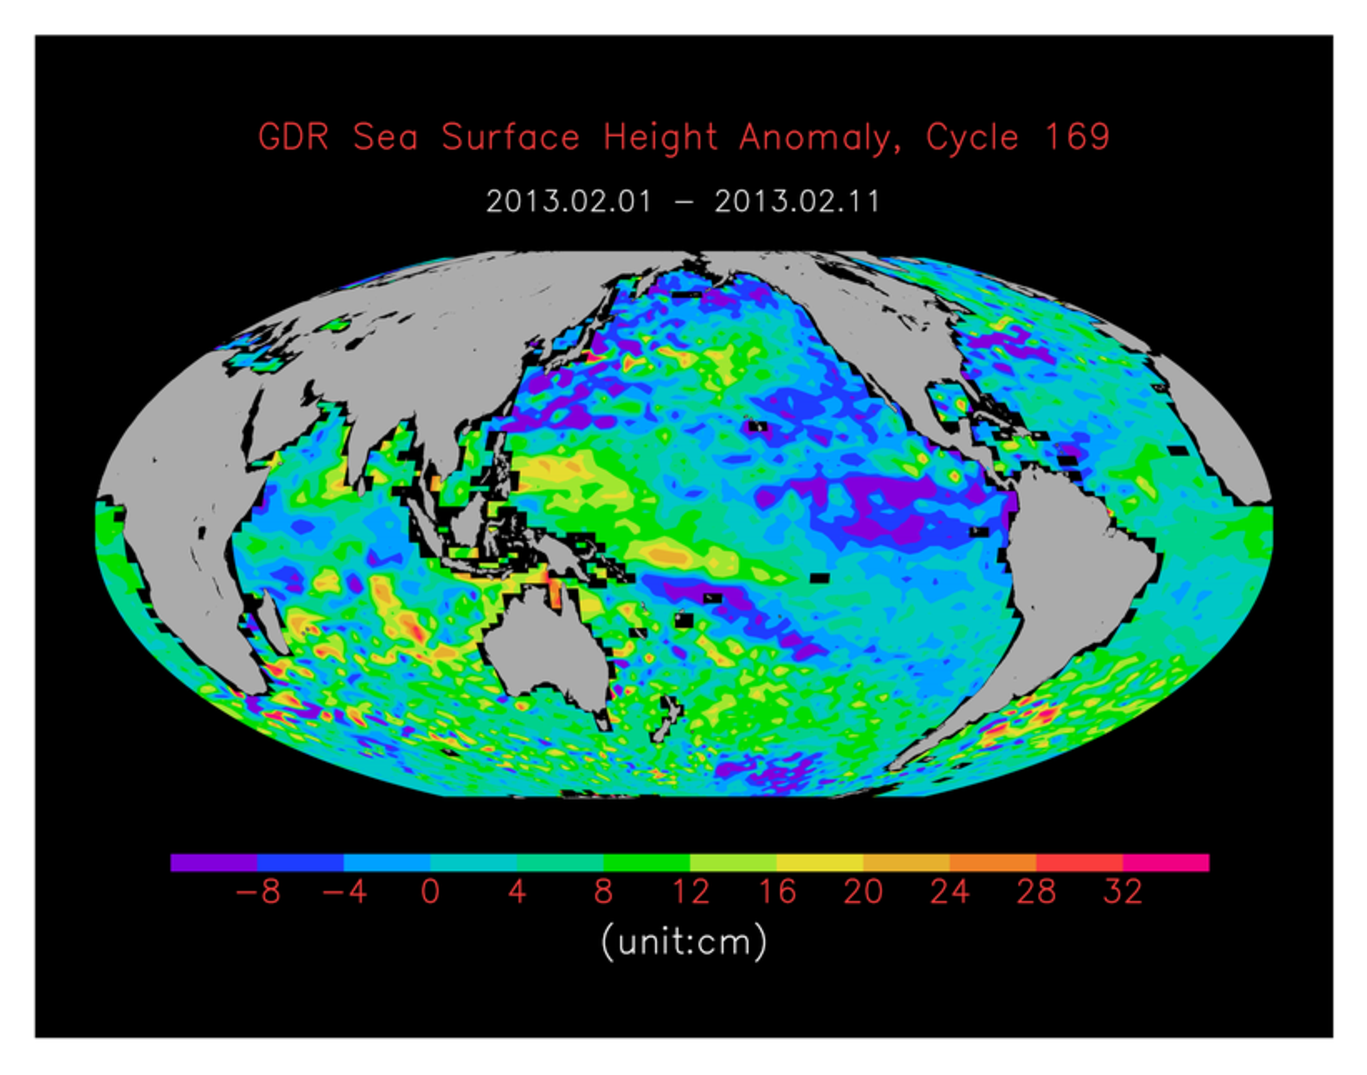
\includegraphics{gdr_ssha_100.eps}}
NOAA

\end{frame}

\begin{frame}
\frametitle{Special Case: Density Constant}

\textcolor{red}{(Exercise: Consider the implications of geostrophic, homogeneous flow, particularly if the bottom of the ocean is not flat)}
\end{frame}

\begin{frame}
http://ocw.mit.edu/courses/earth-atmospheric-and-planetary-sciences/12-003-atmosphere-ocean-and-climate-dynamics-fall-2008/labs/lab6/
\end{frame}

\begin{frame}
\frametitle{Thermal Wind Equations}
\textcolor{red}{(Exercise:Assuming geostrophy and hydrostatic, determine the vertical shear of the horizontal velocity.  That is, $\dudz$ and $\dvdz$.)}

From these equations we can find the velocity at any depth, provided we know it at one depth.
\end{frame}

\begin{frame}
\frametitle{\textcolor{red}{Computer Room Exercise \#1}}

 Use provided code to calculate the velocity through the Florida Straits in balance with the measured density field. Consider different levels of no motion and a ``known'' surface height difference.

\resizebox{2.in}{!}{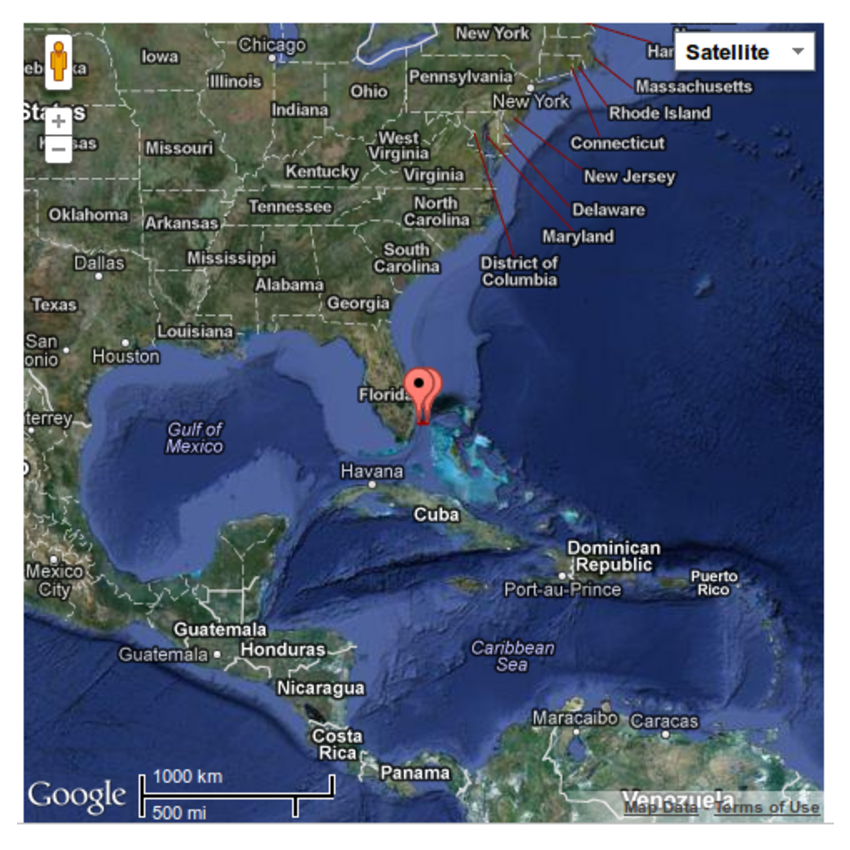
\includegraphics{florida_map.eps}}
\resizebox{2.3in}{!}{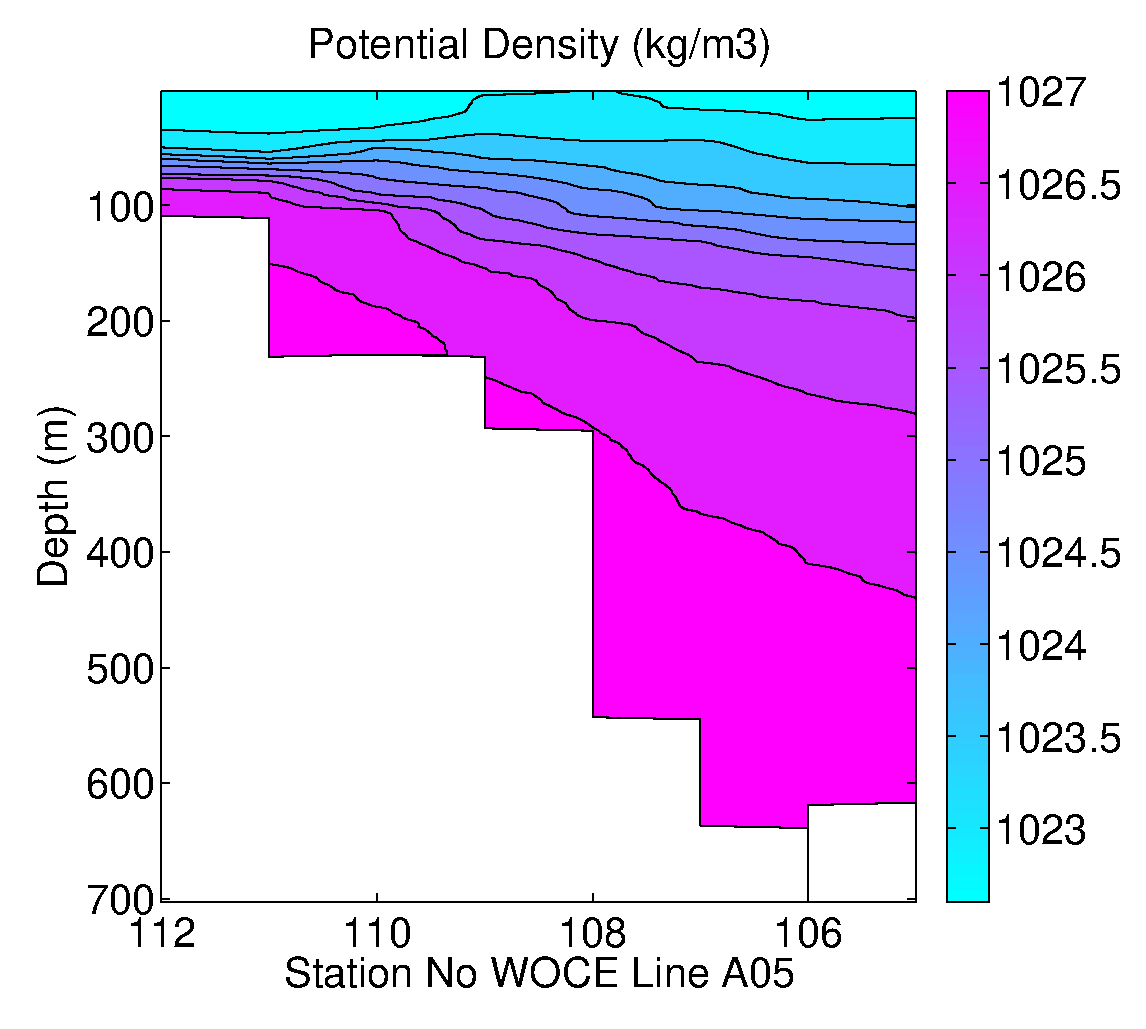
\includegraphics{florida_density.eps}}

{\small Left: Google Maps Right: SEA using data from WOCE}
\label{florida_straits_1}
\end{frame}

\begin{frame}
\frametitle{Thermal Wind Calculation}
\resizebox{2.3in}{!}{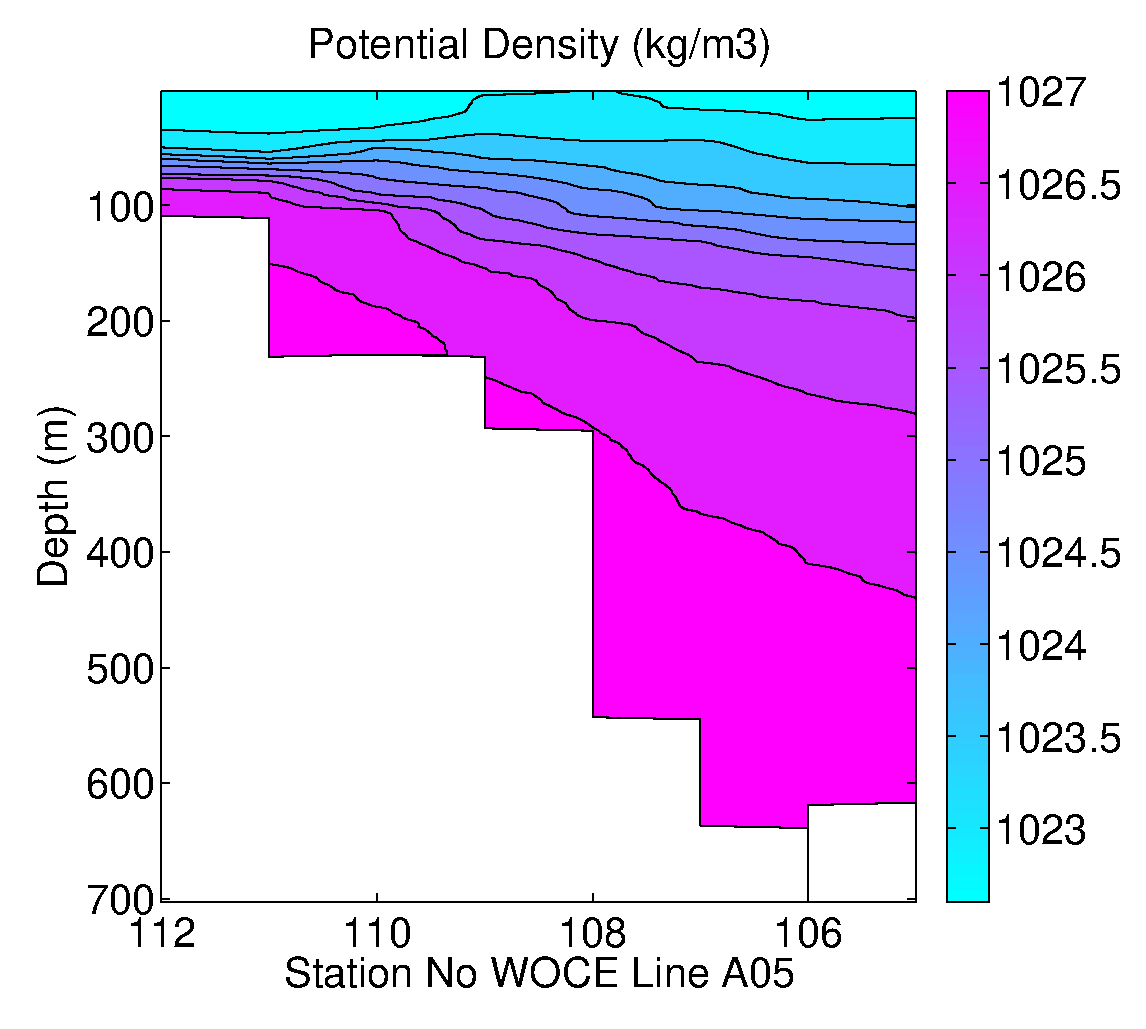
\includegraphics{florida_density.eps}}
\resizebox{1.9in}{!}{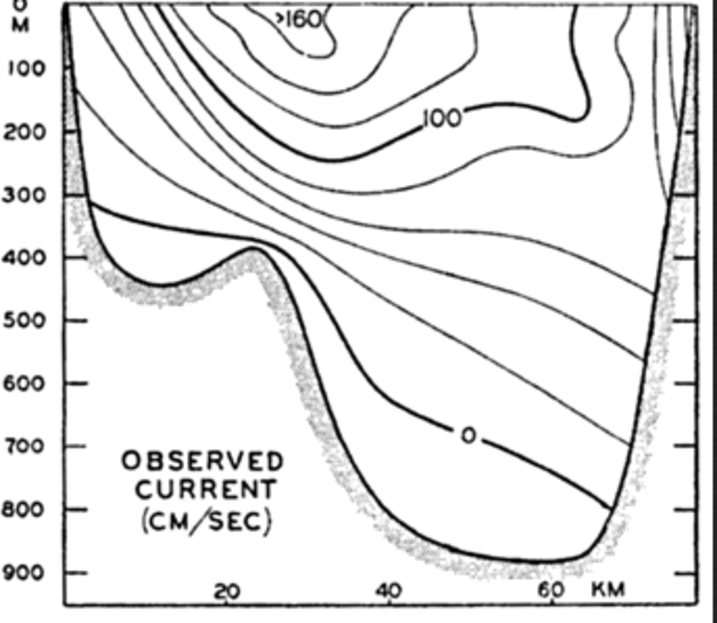
\includegraphics{wust1935.pdf}}

{\small Left: SEA w data from WOCE, Right: Sverdrup et al, 1942.  Note that latter is different time and perhaps different cross-section and hand-contoured}
\label{florida_straits_2}
\end{frame}

\section{5.3 Quasi-geostrophy}

\begin{frame}
\frametitle{More than Geostrophy}

\begin{itemize}
\item The geostrophic equations are degenerate.  We need more terms!

\item The next order terms in the momentum equations are those with $Ro$ and then $Ro_t$ 

\item $Beta$ is smaller but important for larger scale processes.
\end{itemize}

\end{frame}

\begin{frame}
\frametitle{Momentum Equations including Next Order Terms, Non-dimensional}

Tildes dropped

\[
Ro_t \dudt + Ro \left( u\dudx + v\dudy \right) - v - Beta\, y v = -\dpdx 
\]
\[
Ro_t \dvdt + Ro \left( u\dvdx + v\dvdy \right) + u + Beta\, y u = -\dpdy 
\]
\[
\dpdz = \rho
\]
No other terms are significant within an order of 30 in the vertical momentum equation.

\end{frame}
\begin{frame}
\frametitle{The Assumption}

We will write $u = u_g + \epsilon u_a$ and $v = v_g + \epsilon v_a$ where $u_g,v_g$ is the geostrophic velocity, that exactly balances the pressure gradient term.

And we will formally assume that all of $Ro, Ro_t$ and $Beta$ are of size $\epsilon$.  

\vspace{0.2in}

\textcolor{red}{(Exercise: Substitute the expansion for $u$ and $v$ and the approximation for the non-dimensional numbers.  Verify that the equations are solved to order one.  Find the order $\epsilon$ equation.  Solve for $v_a$ and $u_a$.)}
\end{frame}

\begin{frame}
\frametitle{Conservation of Volume, Density, Vertical Momentum}
\label{density_eqn}
\[
\dudx + \dvdy + \frac{Ro_t}{Bu} \dwdz = 0
\]
where we have used the scale equivalences on page 12 and $Bu = |N^2|Z^2/f_o^2X^2$ is order 1. \textcolor{red}{(Exercise: verify that Bu is order 1 and that this equation is exactly solved at order 1)}
\[
\drhodt + \frac{Ro}{Ro_t} \left( u \drhodx + v \drhody \right) - \tilde N^2 w = 0
\]
\textcolor{red}{(Exercise: Taking Bu as 1, substituting the expansion for $u$ and $v$, eliminate w between these equations and using the hydrostatic equation, eliminate $\rho$)}

\end{frame}
\begin{frame}
\frametitle{Merging}

In front of you, you have equations for $u_a$, $v_a$  in terms of the $u_g, v_g$ and $p$ from the horizontal momentum equations and for the horizontal divergence of $u_a$, $v_a$ in terms of the $u_g, v_g$ and $p$ from conservation of volume, density equation and hydrostatic equation.

You could now, differentiate the first two and substitute into the third to get an equation only in $u_g, v_g$ and $p$.  Then substituting the geostrophic velocties written in terms of the pressure, you get one equation in $p$.

\[
\left[ \ddt + \dpdx \ddy - \dpdy \ddx\right] \left[ \nabla_h^2 p + \ddz \left( \frac {1}{\tilde N^2} \dpdz \right)\right] + \dpdx = 0\]
where $\nabla_h^2 = \pa^2/\dx^2 + \pa^2/\dy^2$.
\end{frame}

\begin{frame}
\frametitle{What is this?}

\textcolor{red}{(Exercise: 
\begin{itemize}
\item Show that the first bracket is equivalent to the Lagrangian derivative ($d/dt$) using advection by the geostrophic velocity.
\item Show that $\nabla_h^2 p$ is the relative vorticity $\dv/\dx - \du/\dy$.
\item Show that the second term in the second bracket is the vertical expansion of the distance between lines of constant density.
\end{itemize}}
The last term on the right-hand side is the northward advection $v_g$ changing the Coriolis parameter.)
\end{frame}

\begin{frame}
\frametitle{With our Non-dimensional Numbers}

If we had included our non-dimensional numbers (letting them all be of order $\epsilon$ but not necessarily equal) we would have gotten:

\[
\left[ Ro_t \ddt + Ro \left(\dpdx \ddy - \dpdy \ddx\right)\right] \left[ \nabla_h^2 p + \ddz \left( \frac {1}{Bu \tilde N^2} \dpdz \right)\right] + Beta \dpdx =0\]

This equation is separable: $p(x,y,z,t) = \Pi(z) \bar p(x,y,t)$

\textcolor{red}{(Exercise: Separate this equation)}


\end{frame}

\section{5.4 Vertical Normal Modes}

\begin{frame}
\frametitle{Vertical Part of Equation}
The vertical part can be written 

\[ \ddz \left( \frac{1}{Bu \, \tilde N^2} \frac {\pa \Pi}{\dz} \right)+ \alpha^2 \Pi = 0 \]

If we assume a flat bottom and that the vertical velocity at the surface of the ocean is also zero our boundary conditions are:
\[ w = 0, \, {\rm at}\, z=0\,{\rm and}\, z=-\tilde H\]

Need to move to $w$
\end{frame}

\begin{frame}
\frametitle{Normal Mode Equation}

From page~\pageref{density_eqn} we see that
\[\tilde N^2 w = \left[ \ddt + \frac{Ro}{Ro_t} \left(\dpdx \ddy - \dpdy \ddx\right)\right] \rho\]
and hydrostatic gives
\[\dpdz = -\rho\]

So the vertical component of $w$, 
\[ w_e = \frac{-1}{\tilde N^2} \frac{\pa\Pi}{\dz}\]

\textcolor{red}{Exercise: show that this implies the equation for $w_e$ is:
\[\frac{\pa^2 w_e}{\dz^2} + \alpha^2 Bu\, \tilde N^2 w_e = 0\]}
\end{frame}



\begin{frame}
\frametitle{\textcolor{red}{Computer Room Exercise \#2}}

Use provided code to find the vertical normal modes for different stratifications.
\begin{itemize}
\item How do vertical changes in stratification change the shape of the modes?
\item Explain why the density and vertical velocity modes look like they do, relative to each other.
\item Relate the density mode and the horizontal velocity modes.
\end{itemize}

\end{frame}


\begin{frame}
\frametitle{One more Mode}

By assuming the upper boundary condition is $w=0$ we eliminated the gravest mode.  

For this mode we need to consider the surface moving.
\[ w = \frac{d\eta}{dt} \, {\rm at}\ z=\eta \approx 0\]
But if the surface is higher, the pressure is higher.
\[ p = \rho_o g \eta \, {\rm at}\ z=0\]
Combining and applying our scaling:
\[ w_e = \frac {|N^2|Z}{g}\Pi\, {\rm at}\ z=0\]
{\it Note that our scaling is out as $w_e \ll \Pi$}
\end{frame}

\begin{frame}
\frametitle{Boundary Conditions in $w_e$}

Now we had
\[ w_e = \frac{-1}{\tilde N^2} \frac{\pa \Pi}{\dz}\]
Differentiate and substitute the differential equation for $\Pi$ gives:
\[ \frac{\pa w_e}{\dz} = Bu \alpha^2 \Pi\]
So our boundary condition in terms of $w_e$ is
\[ w_e = \frac{|N^2|Z}{g \alpha^2 Bu}  \frac{\pa w_e}{\dz} \, {\rm at}\ z=0  \]
\end{frame}

\begin{frame}
\frametitle{``External Mode''}
For this mode $\alpha^2 \ll 1$ and the differential equation can be approximated:
\[\frac{\pa^2 w_e}{\dz^2} = 0\]
which has a solution $w_e = W_o (z+\tilde H)$ where the boundary condition $w_e = 0$ at $z=-\tilde H$ has already been applied.

Applying the surface boundary condition:
\[W_o \tilde H = \frac{|N^2|Z}{g \alpha^2 Bu} W_o\]
which expanding $Bu$ gives
\[ \frac{\alpha^2} {X^2}  = \frac{f_o^2}{g H} \approx \frac{1}{(2000\,{\rm km})^2} \]
or a $c_e = 200$m s$^{-1}$ where $A$ is the scale for $\alpha$

\textcolor{red}{(Exercise: show that for this mode $\Pi$ is approximately constant with depth as are $u_g$ and $v_g$)}
\end{frame}

\section{5.5 Rossby Waves}

\begin{frame}
\frametitle{Quasi-geostrophic Waves}

Writing $\alpha^2$ = $1/R_i^2$ where $i$ is the lengthscale for the i$^{th}$ mode, our horizontal equation is
\[
\left[ Ro_t \ddt + Ro \left(\frac{\pa \bar p}\dx \ddy - \frac{\pa \bar p}\dy \ddx\right)\right] \left[ \nabla_h^2 \bar p - \frac{\bar p}{R_i^2}\right] + Beta \frac{\pa \bar p}\dx =0\]

We will look for linear waves and thus formally assume that $Ro \ll \epsilon$.  

\[
Ro_t \ddt \left[ \nabla_h^2 \bar p - \frac{\bar p}{R_i^2}\right] + Beta \frac{\pa \bar p}\dx =0\]

\textcolor{red}{(Exercise: Show that this equation has solutions of the form $\exp[i(kx+\ell y-\omega t)]$ and find the relation between the frequency $\omega$ and the wave-numbers $k, \ell$)}
\end{frame}

\begin{frame}
\frametitle{Rossby Waves}

These waves occur in both the atmosphere and ocean and explain phenomena such as waves on the Jet Stream, the Gulf Stream and the Agulhas Current.

\textcolor{red}{(Exercise: In what directions can these waves propagate?)}

http://www.youtube.com/watch?v=ELDkYJWHNiU
\end{frame}

\section{5.6 Eddies}

\begin{frame}
\frametitle{Potential Vorticity Form}

Our horizontal equation
\[
\left[ Ro_t \ddt + Ro \left(\frac{\pa \bar p}\dx \ddy - \frac{\pa \bar p}\dy \ddx\right)\right] \left[ \nabla_h^2 \bar p - \frac{\bar p}{R_i^2}\right] + Beta \frac{\pa \bar p}\dx =0\]
can also be written
\[ Ro_t \frac{\pa q}{\dt} + {\cal J}(Ro \bar{p}, q) = 0 \]
where $q = \nabla_h^2 \bar p - \bar p / R_i^2 + (Beta/Ro)\, y$ and ${\cal J}$ is the Jacobian.

\textcolor{red}{(Exercise: Show these relations are equivalent)}
\end{frame}
\begin{frame}
\frametitle{Compact, Steadily Translating Eddy}

We will assume that $\bar{p} = \bar{p}(x-ct,y)$ and that $\bar{p}$ is compact in form.  As $x$ and $t$ only occur combined, we can include the time-derivative in the Jacobian and assume $Ro == Ro_t$
\[ {\cal J}(\bar{p} + c y, q) = 0\]
which has a solution $q = {\cal F}(\bar{p} + cy)$ for some function ${\cal F}$.

We can assume two types of contours of $\bar{p}$.  

1) Those that are closed near the center of the eddy $r < a$ which we will ignore for now.
  
2) Those that extend to great distances.  A long way from the eddy $q$ should approach $(Beta/Ro)\, y$ as the eddy has compact form and $\bar p$, the perturbation pressure, should vanish.  Thus along these contours, ${\cal F}$ should be linear, that is ${\cal F}(\gamma) = (Beta/Ro) \gamma/c$. 

\end{frame}

\begin{frame}
\frametitle{Eddy Solution}

So in the outer region we have an equation
\[ \nabla_h^2 \bar{p} - \frac{1}{R_i^2}\bar{p} = \frac{Beta}{Ro\, c} \bar{p}\]
which boundary condition that $\bar p \rightarrow 0$ at large distance from the origin and constant at $r = a$.

\textcolor{red}{Exercise: Show that 
\[ \bar{p} =P_o K_o (mr) \]
is a solution, where $K_o$ is the gravest modified Bessel function and where
\[ m^2 = \frac{1}{R_i^2} + \frac{Beta}{Ro\, c}\]}

\end{frame}

\begin{frame}
\frametitle{``Ocean Eddy''}

\resizebox{0.7\textwidth}{!}{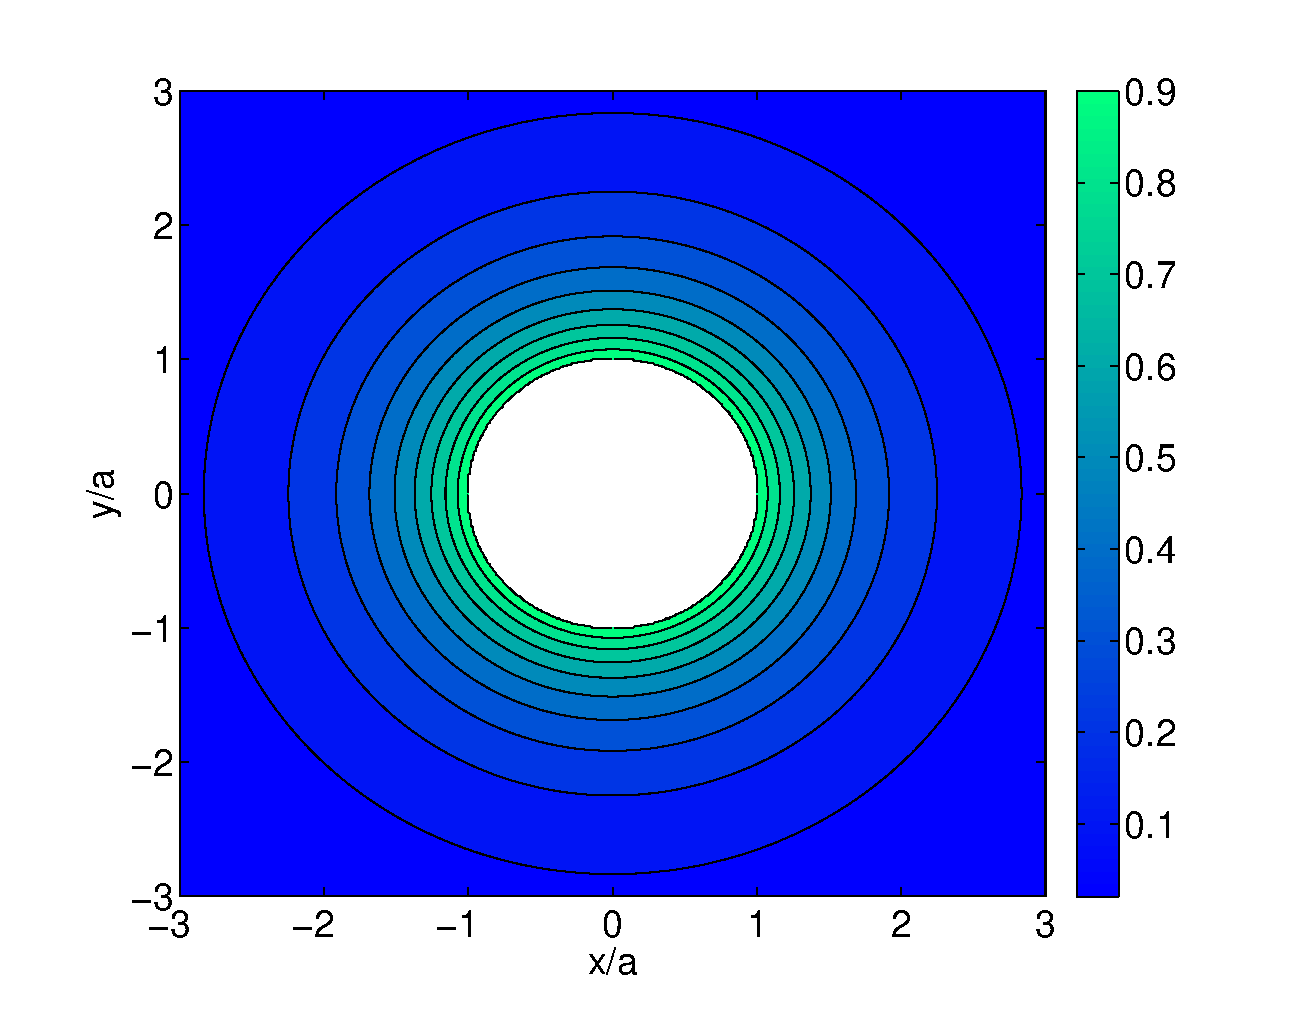
\includegraphics{eddy.eps}}SEA

\textcolor{red}{(Exercise: Given that $m$ is real, what real values can $c$ take?)}

\textcolor{red}{(Exercise: what direction to eddies large compared to $R_i$ move?  Small?)}
\end{frame}

\begin{frame}
\frametitle{Theme Movie and Image Credits}

{\bf Movie}\\
http://www.nasa.gov/topics/earth/features/perpetual-ocean.html

\vspace{0.5in}

{\bf Image Credits}
\begin{itemize}
\item Theme Movie \& Still: NASA: {\tiny http://www.nasa.gov/topics/earth/features/perpetual-ocean.html}
\item Sea Surface Height, page~\pageref{ssh_image} NOAA: {\tiny www.nodc.noaa.gov/sog/Jason2/qa.html}
\item Map: page~\pageref{florida_straits_1} Google Maps
\item Right Contour Plot, page~\pageref{florida_straits_2} Sverdrup, H.U., M.W. Johnson and R.H. Fleming.  The Oceans, their Physics, Chemistry and General Biology. Prentice-Hall, INc. 1942. 
\end{itemize}

\end{frame}

\end{document}